\section{Cartoon of Algorithm}
\label{AlgCartoon}

Refer to Fig. \ref{fig:cartoon}.

\begin{figure}
\begin{center}
\scalebox{1}{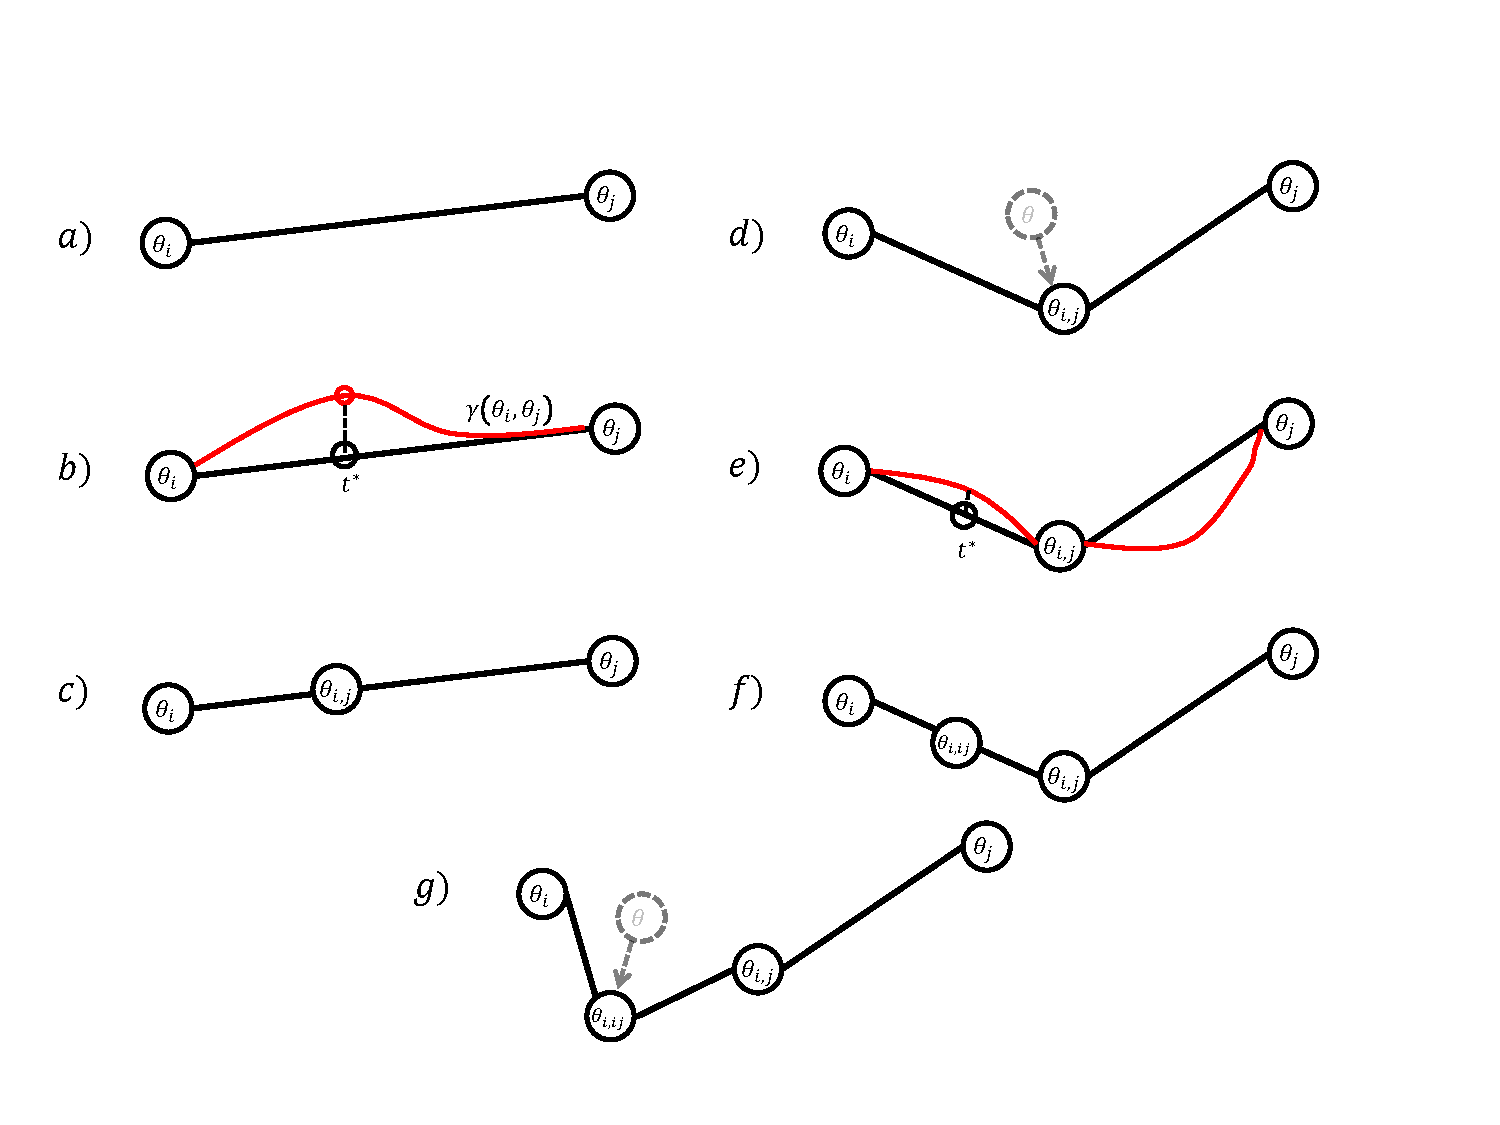
\includegraphics[width=1.0\textwidth]{../AlgorithmFigure}}
\end{center}
\caption{A cartoon of the algorithm.  $a):$ The initial two models with approximately the same loss, $L_0$. $b):$ The interpolated loss curve, in red, and its global maximum, occuring at $t=t^*$. $c):$ The interpolated model $\Theta(\theta_i, \theta_j, t^*)$ is added and labeled $\theta_{i,j}$.  $d):$ Stochastic gradient descent is performed on the interpolated model until its loss is below $\alpha L_0$. $e):$ New interpolated loss curves are calculated between the models, pairwise on a chain.  $f):$ As in step $c)$, a new model is inserted at the maxima of the interpolated loss curve between $\theta_i$ and $\theta_{i,j}$.  $g):$  As in step $d)$, gradient descent is performed until the model has low enough loss.}
\label{fig:cartoon}
\end{figure}


\section{Visualization of Connection}
\label{visualization}

 Because the weight matrices are anywhere from high to extremely high dimensional, for the purposes of visualization we projected the models on the connecting path into a three dimensionsal subspace.  Snapshots of the algorithm in progress for the quadratic regression task are indicated in Fig. \ref{connfigs}.  This was done by vectorizing all of the weight matrices for all the beads for a given connecting path, and then performing principal component analysis to find the three highest weight projections for the collection of models that define the endpoints of segments for a connecting path---i.e., the $\theta_i$ discussed in the algorithm.  We then projected the connecting string of models onto these three directions.  
 
 The color of the strings was chosen to be representative of the test loss under a log mapping, so that extremely high test loss mapped to red, whereas test loss near the threshold mapped to blue.  An animation of the connecting path can be seen on our \href{github.com/danielfreeman11/convex-nets/blob/master/Writeup/Plots/quadratic.pathinterp.errorvis.gif}{Github page}.
 
 Finally, projections onto pairs of principal components are indicated by the black curves.
 
\begin{figure}
\label{connfigs}
\centering
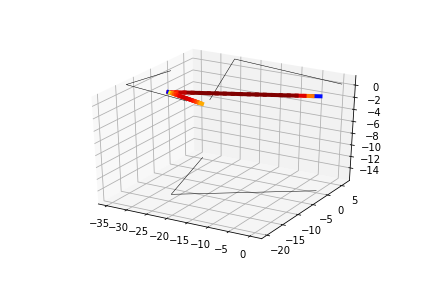
\includegraphics[width=.4\textwidth]{../Plots/conn1}
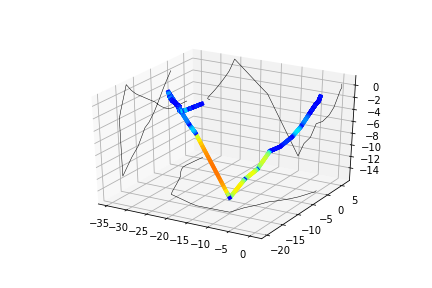
\includegraphics[width=.4\textwidth]{../Plots/conn2}
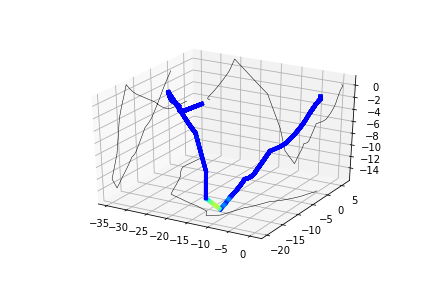
\includegraphics[width=.4\textwidth]{../Plots/conn3}
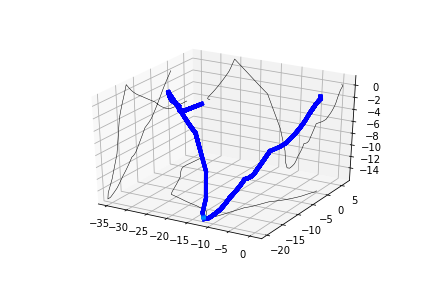
\includegraphics[width=.4\textwidth]{../Plots/conn4}
\caption{Snapshots of Dynamic String Sampling in action for the quadratic regression task.  The string's coordinates are its projections onto the three most important principal axes of the fully converged string.  (Top Left) One step into the algorithm, note the high loss between all of the vertices of the path. (Top Right) An intermediate step of the algorithm.  Portions of the string have converged, but there are still regions with high interpolated loss. (Bottom Left) Near the end of the algorithm.  Almost the entire string has converged to low loss.  (Bottom Right) The algorithm has finished.  A continuous path between the models has been found with low loss.} 
\end{figure}
 
 


\section{A Disconnection}
\label{sec:disconnect}

%%%%%%%%%%%%%%%%%%%%%%
\subsection{A Disconnection}
%%%%%%%%%%%%%%%%%%%%%%
\label{symdisc}

 As a sanity check for the algorithm, we also applied it to a problem for which we know that it is not possible to connect models of equivalent power by the arguments of section \ref{disconnect}.  The input data is 3 points in $\mathbb{R}^2$, and the task is to permute the datapoints, i.e. map $\{x_1,x_2,x_3\} \to \{x_2,x_3,x_1\}$.  This map requires at least 12 parameters in general for the three linear maps which take $x_i\to x_j$ for $i,j \in \{\{1,2\},\{2,3\},\{3,1\}\}$.  Our archticture was a 2-3-2 fully connected neural network with a single relu nonlinearity after the hidden layer---a model which clearly has 12 free parameters by construction.  The two models we tried to connect were a single model, $\theta$, and a copy of $\theta$ with the first two neurons in the hidden layer permuted, $\tilde{\theta_{\sigma}}$.  The algorithm fails to converge when initialized with these two models.  We provide a visualization of the string of models produced by the algorithm in Fig. \ref{discfigs}.
 
 In general, a persistent high interpolated loss between two neighboring beads on the string of models could arise from either a slowly converging, connected pair of models or from a truly disconnected pair of models.  ``Proving'' a disconnection at the level of numerical experiments is intractable in general, but a collection of negative results---i.e., failures to converge---are highly suggestive of a true disconnection.
 
\begin{figure}
\label{discfigs}
\centering
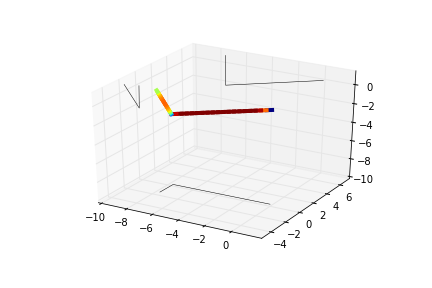
\includegraphics[width=.4\textwidth]{../Plots/disc1}
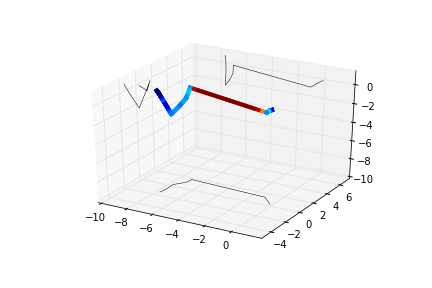
\includegraphics[width=.4\textwidth]{../Plots/disc2}
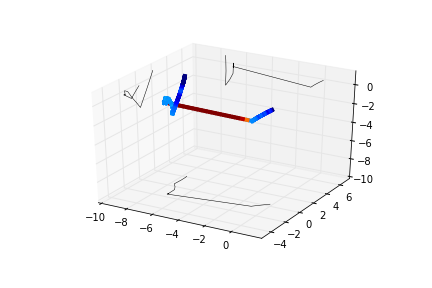
\includegraphics[width=.4\textwidth]{../Plots/disc3}
\caption{These three figures are projections of the components of the 12-dimensional weight matrices which comprise the models on the string produced by the DSS algorithm.  The axes are the principal components of the weight matrices, and the colors indicate test error for the model.  For more details on the figure generation, see Appendix \ref{visualization}. (Left) The string of models after 1 step.  Note the high error at all points except the middle and the endpoints.  (Middle) An intermediate stage of the algorithm.  Part of the string has converged, but a persistent high-error segment still exists.  (Right) Even after running for many steps, the error persists, and the algorithm does not converge.}
\end{figure}